
\chapter{POND Evaluation}
\label{cha:cont4}
The previous in-lab study (the comparison between BAL-HEI-FBQI) clarified that some people preferred the detailed calorie lookup, while some were satisfied with the checkbox approach, which was in contrast to what we expected based on the BALANCE study, where many participants reported frustration with the BALANCE tool. This chapter presents the results of an evaluation of the POND tool described in the previous chapter. The reported results focus on what people entered, when they made entries and how it changed over time, and how they chose to create the entries.  

\section{Introduction}
The POND evaluation included both in-lab and \textit{in situ} components.  The in-lab study was similar in design to the BAL-HEI-FBQI study presented in Chapter \ref{cha:app_cont2_inlab_surveys}. Participants came to the lab, used the POND tool to make food entries specified on a card, then asked for feedback about the tool and experience. The in-lab portion was piloted, and the software was modified based on feedback from participants. The \textit{in situ} component had participants install the POND software on their  personal phone, and to use it to track what they eat for three weeks. 

I present the two studies in two sections: The first reflects the in-lab portion of the studies, and the second focuses on the real-world portion of the study. The in-lab portion of the study were the same (same data collected, same tasks used), with minor changes to the software between phases. 

One area of interest in this study was how people would personalize the POND software to make it personally interesting, important, and not too challenging. The in-lab portion of the study consisted of conditions that varied the number of components on the screen. This was to introduce participants to the idea of varying complexity and the customization. We believed that participants who could personalize the tool to something that fit within their goals, motivation and resources would be more satisfied with using the POND software to monitor their food intake. 

\section{Evaluation Organization}
This evaluation consisted of an in-lab pilot, then an in-lab and in situ  data collection. The software was slightly modified based on feedback from the participants in the pilot, then used for the rest of the study. The second part of the study consisted of participants performing the same tasks as in the pilot in-lab study, followed by them tracking their dietary intake using POND on their personal mobile phone. 

I report and discuss the data in terms of the in-lab portion and the in situ data. When discussing the in-lab data, I treat the pilot and final data in the same way. 

First, I describe the in-lab part of the study. Then, I describe the data collected, report the results and discuss. Next, I describe the in situ part of the study, the data collected in situ, report the results and discuss. Then, I discuss overall, addressing anything that is related between the in-lab and in situ portions. 

\section{In-Lab Evaluation}
\label{sec:inlabEval}
The purpose of the in-lab evaluation is to collect data to characterize how people use the POND software to enter known food tasks. 

\subsubsection{Research Questions/Goals}
There were two primary goals with this in-lab study. First was to collect data to characterize what kinds of errors people made when entering known food into the software, and second was to collect formative feedback on the concept of using POND to support setting and monitoring small goals. 

\subsection{Experiment Design}
This in-lab evaluation is a single-factor, multilevel, within-subjects design. The single factor is the number of components enabled in the POND interface. There are four levels: Small (2 components), Medium (5 components), Large (9 components) and Full (all 13 components). The components for each condition were chosen randomly (without replacement) for each participant at the start of the study. All components were used at least once. Condition order was counterbalanced, and tasks were always presented in the same order. All of the target amounts for each component were calculated by the HEI-05 recommendations for an adult with a target calorie intake of 2000 calories. 


\subsubsection{Procedure}
After completing the informed consent, participants were asked to complete a questionnaire to report demographics and background information, such as familiarity with mobile phones (including text entry), experience with using food diaries on different platforms (paper, web, mobile phone), and general health and wellness goals. 

Participants were briefed on the concept and benefits of a dietary pattern, and informed about the HEI-05 and all of the individual components. This information was similar to the details provided in the POND app (via the ``More details...'' button), but more detailed. A printed version was provided for reference. The app was explained to the participant, and some example entries were made. The participant was given time to use the app individually and ask any questions. 

The study consisted of 4 series of 5 tasks: 4 conditions with 5 tasks in each condition. Each condition represented roughly 1 day of food intake, with each task representing the content of 1 meal. Each task was presented on a card, with a single food on each line, and the amount printed below. Task cards had printed IDs, and the software was modified to ensure that input aligned with the correct task. For each task, participants were instructed to start the app and enter the food as desired (using either the +1 buttons or the database lookup), and hit the back button to exit the app when all foods on the card were entered.  At the end of each condition, participants completed a questionnaire that included TLX measures. 

Participants were asked to tell the administrator if they made a mistake, but not to fix it. The app was designed such that entering was very easy, but fixing a mistake took longer. For this study, we wanted to be able to capture the entry time not confounded by edit time. This approach allowed us to capture the distinction between an error the participant knew they made, and errors they were unaware of. 

At the end of all four conditions, participants completed a questionnaire that focused on overall feedback about the software. 
\begin{figure}	
\centering
	\begin{subfigure}[t]{1.25in}
		\centering
		\setlength\fboxsep{0pt}
\setlength\fboxrule{0.5pt}
\fbox{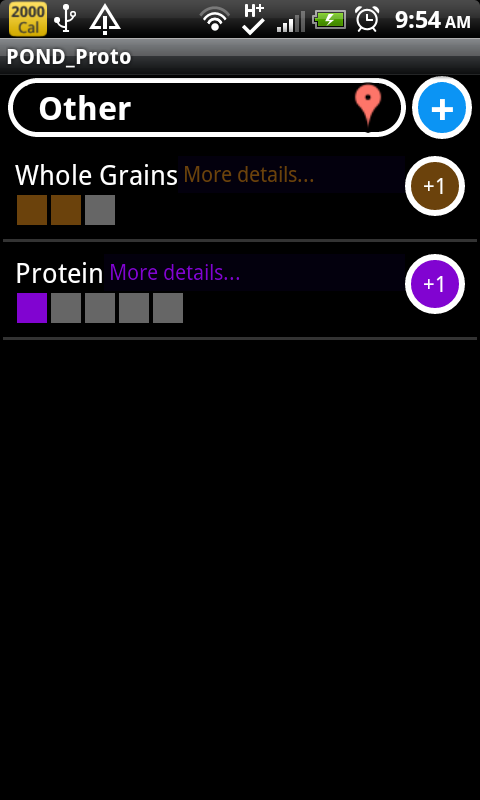
\includegraphics[width=1.25in]{./images/cont4/small_condition}}
		\caption{Small condition.}\label{fig:small_cond}
	\end{subfigure}
\quad
\begin{subfigure}[t]{1.25in}
		\centering
		\setlength\fboxsep{0pt}
\setlength\fboxrule{0.5pt}
\fbox{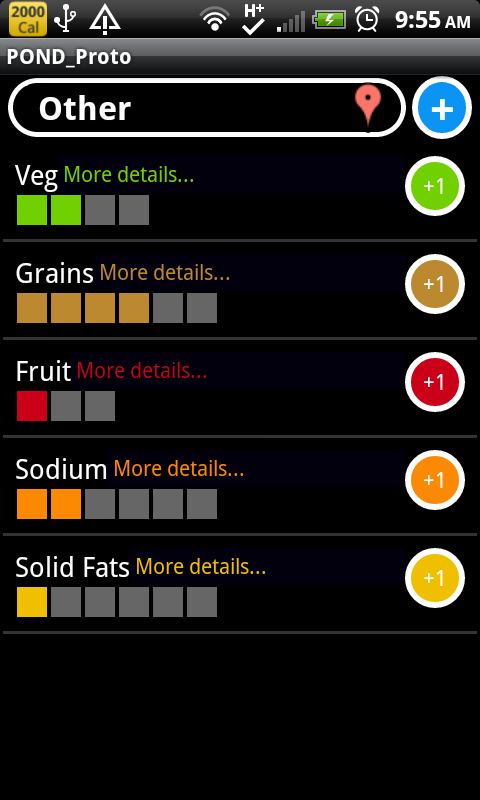
\includegraphics[width=1.25in]{./images/cont4/medium_condition}}
		\caption{Medium condition. }\label{fig:med_cond}
	\end{subfigure}
\quad
\begin{subfigure}[t]{1.25in}
		\centering
		\setlength\fboxsep{0pt}
\setlength\fboxrule{0.5pt}
\fbox{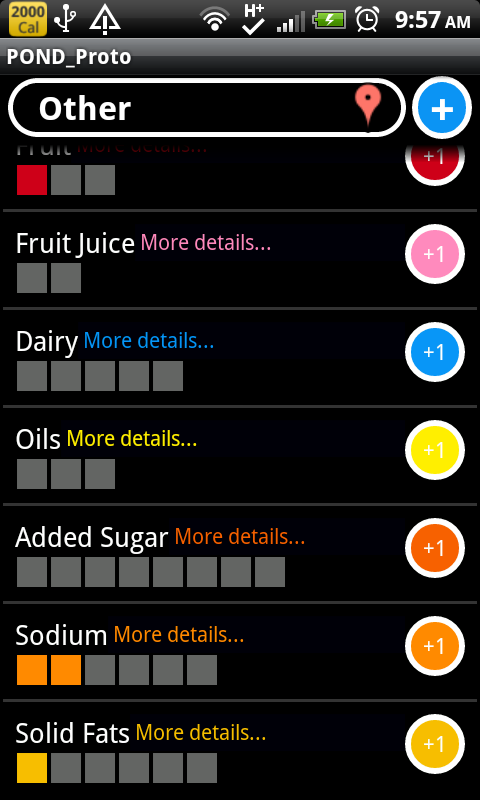
\includegraphics[width=1.25in]{./images/cont4/large_condition}}
		\caption{Large condition. }\label{fig:large_cond}
	\end{subfigure}
	\caption{POND Home screens for each condition}\label{fig:3_1}
\end{figure}



\subsubsection{Tasks}
The tasks were the same as developed for the in-lab study reported in Chapter \ref{cha:app_cont2_inlab_surveys}. However, the tasks were developed using an earlier version of the food database (Nutritionist Pro Knowledge Base, Version 4.2) than was used for the POND app (Nutritionist Pro Knowledge Base, Version 4.4). One major modification from Version 4.2 to Version 4.3 was the ``Food Naming System''. New food names had a different ordering strategy than the previous one. An example is in Version 4.2, example food entries are ``Mashed Potatoes'' and ``Reduced Fat Milk, 2\%'', while corresponding entries in Version 4.3 (and later) are ``Potatoes, Mashed'' and ``Milk, Reduced Fat 2 \%''. The task cards had the Version 4.2 food names, so participants were looking for ``Mashed Potatoes'', but had to choose ``Potatoes, Mashed''. This could arguably more closely reflect a real world experience, where the individual needs to generate a query term.

\subsubsection{Participants-- Pilot}

12 participants were recruited from email lists for a major university. All participants were students or instructors in a technology-centric field (Computer Science \& Engineering, Informatics,  and Human-Centered Design \& Engineering). 6 male, 6 female.  All reported using a cell phone several times a day, and all but one reported entering text on their cell phone several times per day (the other one reported entering text on their cell phone 1-2 times per day). All participants owned smartphones, 2 participants owned smartphones that did not have a touch-screen and 4 owned smartphones with QWERTY keyboards. 4 reported using a food diary previously. Of the 4, all had used a food diary on a smartphone, while one of those 4 had also used paper and either software or a website. When asked about health concerns and goals, 11 people indicated that they are interested in ``eating better'', 6 are interested in losing weight, 2 want to better control portion sizes, and 2 are interested in eating less or more. Other answers volunteered included ``Eating fewer processed foods'', and ``Eating only healthy/no junk food''. When asked to rate on a scale of 1-4 (very knowledgeable) how knowledgeable they are about food and nutrition (``including nutrients (fat, carbohydrates, fiber, vitamins, etc) and/or ingredients''), 5 reported themselves as a 2, 6 reported themselves as a 3, and 1 reported themselves as 4, or that they ``are expert/have spent much time understanding nutritional aspects of food.''

Participants were compensated for their time with a \$10 Amazon gift certificate.

\subsubsection{Participants}

22 people participated in this study, 17 female and 5 male. Ages ranged from 21-64, and occupations varied. All participants reported using their cell phone several times a day, and all except 1 reported entering text on their cell phones several times a day (the remaining one entered text on their cell phones 1-2 times daily). All participants owned cell phones with touch screens, and 2 owned phones with an additional QWERTY keyboard. 19 participants reported that one of their health goals is to ``Eat better'', while 8 reported wanting to lose weight, 8 wanted to better control portion sizes, and 4 wanted to eat less or more. 6 people reported never tracking their food intake before, while 7 had used a smart phone, 8 had used a website, 8 had used paper, and 1 used some other software on their computer. 7 reported themselves as very knowledgeable about food and nutrition, 10 as fairly knowledgeable, 4 as not so knowledgeable, and 1 as fairly uneducated about food and nutrition.  

Participants were recruited from the community via craigslist posting, a recruitment request sent to a local mom email list, posters in the neighborhoods at cafes, bookstores, and athletic shops, as well as some email lists at the university that were different than the ones used in previous studies. Participants were compensated \$125 for their complete participation in the study. Participants self-reported that they had no medical concerns that impacted their food choices, and owned their own Android devices. 

Four participants completed the in-lab part, but did not complete the in situ part of the study. Of the four, two were unable to install the software on their personal devices, and two chose not to continue the study. 

\subsection{Measures and Data Collected}
\begin{enumerate*}
\item \textbf{Entry Strategy.} How a task was entered: with just +1 buttons, just lookup, or a mix of the two. 
\item \textbf{Correctness/Errors. } A score from 0-2 representing the correctness the task entry. 
\item \textbf{Timing/duration.} Time spent in each condition. 
\item \textbf{TLX.} TLX \citep{Hart2006} measures reported after each condition. 
\item \textbf{Likes/dislikes} List of self-generated features liked and not liked about each condition. 
\item \textbf{Search terms.} A list of the searches executed for each task/food item. 
\item \textbf{Final questionnaire.} Includes questions about how likely the participant is to use the app for a given length of time, and how interesting and useful each individual component is. The entire questionnaire is documented in the Appendix. 
\end{enumerate*}


\subsubsection{Study Design Limitations}
As noted in Chapter \ref{cha:relatedWork}, the process of using written food names as tasks has the potential to include foods participants may not be familiar with. This is addressed by asking participants to report their familiarity with the foods at the end of each condition. The scripted nature of the study prevented participants from exploring features of the software and becoming more familiar with it. As with most food diaries, POND is designed to be quicker and easier over an extended period of use, thus in-lab studies may reflect the novice effect. Finally, all food diaries evaluated in a lab setting do not reflect the reality that  situation and context matter when using a food diary in situ. 

\subsection{Results}

\subsubsection{Component Counts}
I'm not sure if I need this section, or exactly what needs to go here. This addresses the ``what'' question: what did people enter? But really, it gets more back to correctness. There is no other meaningful way to summarize or present this. Each participant entered the same task, but each participant had a different set of components to enter for the task. People could legitimately not enter components. 

I have an image that displays ground truth of each task and each participants results, for each task. That would be too unwieldy. 


\subsubsection{Entry Strategy}
Entry strategy reflects how participants made entries. In general, we were interested in when people made the decision to use the +1 buttons or the lookup feature to enter a food. We found participants tended to have their preference for using +1 or lookup. The results are summarized in \ref{tab:inlab_strategy}. 

In the table, ``Only +1'' and ``Only Lookup'' mean that the participant only used the +1 or lookup entry process, respectively. The ``Mostly'' designation reflects that a majority of the entries were made with the specified process. ``Mix'' did not reflect a strong preference for either strategy. 


% Table generated by Excel2LaTeX from sheet 'PONDstrategy_inlab'
\begin{table}[htbp]
\small
  \centering
  \caption{Entry Strategy}
    \begin{tabular}{rrrr}
    \toprule
          & Num Pilot Ppts & Num Ppts & Total \\
    \midrule
    Only +1 & 3 (25\%) & 7 (29\%) & 10 (28\%) \\
    Mostly +1 & 1 (8\%) & 3 (13\%) & 4 (11\%) \\
    Mix   & 1 (8\%) & 10 (42\%) & 11 (31\%) \\
    Mostly Lookup & 4 (33\%) & 4 (17\%) & 8 (22\%) \\
    Only Lookup & 3 (25\%) & 0 (0\%) & 3 (8\%) \\
\midrule
    Total & 12 (100\%) & 24 (100\%) & 36 (100\%) \\
    \bottomrule
    \end{tabular}%
  \label{tab:inlab_strategy}%
\end{table}%


 \textbf{Pilot data:}
Three participants chose to use the +1 buttons exclusively, while one other participant used the +1 buttons primarily, but tried the lookup function a bit. Of the remaining 8 participants, 4 mostly used the lookup function, 1 used lookup or a combination exclusively, and the last 3 used a combination of the three strategies. 

\textbf{data:}
Seven participants chose to use the +1 buttons exclusively, while three other participants used the +1 buttons primarily, but tried the lookup function a bit. Of the remaining 14 participants, 4 mostly used the lookup function,  none used lookup or a combination exclusively, and the last 10 used a combination of the three strategies. 


\subsubsection{Search Terms}
% Table generated by Excel2LaTeX from sheet 'search terms'
\begin{table}[bthp]
\small
  \centering
  \caption{Common queries}
    \begin{tabular}{rr}
    \toprule
    Query term & Number of people who used it \\
    \midrule
    doritos & 11 \\
    baking chocolate & 10 \\
    egg   & 10 \\
    wheat thins & 9 \\
    fiber one & 9 \\
    pepperoni & 9 \\
    starbucks & 9 \\
    mashed potatoes & 8 \\
    wheat crackers & 8 \\
    don miguel & 8 \\
    le gout & 8 \\
    salad & 8 \\
    milk  & 8 \\
    \bottomrule
    \end{tabular}%
  \label{tab:inlab_commonqueries}%
\end{table}%


% Table generated by Excel2LaTeX from sheet 'search terms'
\begin{table}[htbp]
\small
  \centering
    \begin{tabular}{rrrr}
    \toprule
    description & Number of people who used it &       & length  \\
    \midrule
    pauly county line advantage swiss cheese & 1     &       & 40 \\
    pepperidge farm crusty Italian garlic & 1     &       & 37 \\
    bag n season pork chop seasoning mix & 1     &       & 36 \\
    keebler zesta soup \& oyster crackers & 1     &       & 36 \\
    low calorie thousand island dressing & 1     &       & 36 \\
    pepperidge farm crusty utilian bread & 1     &       & 36 \\
    \bottomrule
    \end{tabular}%
  \caption{Long queries}
  \label{tab:inlabLongQueries}%
\end{table}%


When participants chose to make food entries by using the food database, they generated a query. For the non-pilot study, we saved all of the search terms and report on them here. Terms that appeared to be part of the practice tasks were excluded. 

Overall, the 24 non-pilot participants made 650 queries from 273 unique phrases. 130 query terms were used by more than one person. All phrases with 8 or more queries are listed in Table \ref{tab:inlab_commonqueries}. Of these 13 queries, 3 represent foods that most likely fit into a single category (egg, salad and milk). It is possible that the salad query was used to find a ``Caesar salad'' entry (salad greens plus dressing and croutons), rather than simply salad greens, which could be counted with just one food group. The other 10 most common queries represent foods that are primarily packaged and prepared. The 6 longest queries are listed in Table \ref{tab:inlabLongQueries}. The mean length of query is 13.6 characters. 

\subsubsection{Likes and Dislikes}
Participants were asked to provide 3 things they liked and disliked about the interface after each condition. Here, the responses are summarized and some common themes identified. Since the presentation of the different conditions was counterbalanced, the comments reflect that some participants saw the conditions growing or reducing from condition to condition. Also, comments in regards to the 

\textbf{SMALL CONDITION}
Some people liked that it was so short (``it was trying to just keep track of my best and worst food choices''), while others felt it was too limiting ``I wanted to put all of the food I ate into categories, not just some of it''. 

\textbf{MEDIUM CONDITION.}
Fewer items, so it takes less time, but more ``mentally taxing'', because they ``had to think more about whether a food contained parts of the specified categories''. One person mentioned s/he liked ``Quicker entry for foods I've encountered before''. 

\textbf{LARGE CONDITION.}
Most comments are similar to the other conditions. A couple stand out as relevant to this condition: ``I don't find any different approach with the first approach, I just realize that there is no meat nutrients therefore everytime [sic] i see meat then i will just skip it.'' ``Didn't feel much difference between the first and second approach. However, I did like that there were different categories.''

\textbf{FULL CONDITION.}
Liked having all the categories. Liked that it made them more informed, covering all the parameters. 

\textbf{OVERALL/APPLIES TO ALL CONDITIONS}
Database-having so many items, but not ``all items sold in stores''. No easy undo (limitation of the study protocol). Liked the ability to search overall. Learning curve to figuring out what food falls into what category. Liked color coded categories of food, and felt they could learn the components and portion sizes over time. Did not like the lack of feedback or uncertainty of whether something was added correctly. Fun to hit the +1 buttons. Liked the colors, the ``meter''. Search results were too wordy and took too long to find the exact food and portion size. Made me think about the nutritional value of what I'm eating, and it keeps me informed of my habits. Even though it takes too many steps to enter a food item, I'd prefer to specify the food I eat and just get the analysis back. 


\subsection{Discussion-- In lab}

The goal of the in-lab portion of the POND evaluation was to characterize how people used the diary to create known food entries. We looked at the strategy participants used to make an entry, the search terms used for known foods, and the things participants liked and disliked. 

We saw that overall, participants were split on how much to use the +1 buttons rather than the lookup feature for creating food entries. The distribution of strategies people used in the pilot study is different than the strategies people used in the full study. More participants in the pilot utilized the search feature, while participants in the full study relied more on the +1 entry strategy, although they also appeared to be more likely to combine the strategies. However, pilot participants were quite vocal about their negative impression of the search feature, which is why it was modified before the full study. Those pilot participants, who had the poor search implementation, used it much more than the participants who had the revised search function. 

The difference in strategy proportions for pilot and non-pilot could reflect the different populations. The pilot study consisted primarily of graduate students in fairly technical fields, while the study population consisted of people from the general population. 

The randomization of the components to the conditions could impact the choices that participants made in regards to using the +1 versus lookup. The Full condition (which contained all components) are comparable across all participants, but in the Small and Medium conditions, it is possible that the components contain either just easy food groups (Fruit, Veggies) or all nutrients (Sodium, Sugar), which are known to be more challenging to count, and people report using the lookup feature for them.

Reviewing the most common search results indicates that participants are searching for unfamiliar, processed foods that are challenging to identify components for. These foods also tend to be higher in sodium and solid fats, which are difficult to estimate without looking up. The most common searches are one or two words. One thing we are unable to evaluate is if  short searches result in a hit more frequently than long searches. The long searches are very similar to the text that appeared on the task card. This reflects how the task cards prime the users to choose search terms. 

The reported likes and dislikes revealed that for this general population that is not necessarily in the process of changing their eating behaviors, the changing of the components on the home screen is not meaningful. In particular, participants felt it odd that some foods might not be counted at all in a given condition. For example, in the small condition, an apple might not be counted if the two components are `sugar' and `sodium'. This is consistent with feedback in the food index comparison study. However, some people noted that it might be worthwhile to spend a short time focusing on one particular component. Overall, people liked the analysis of the food intake pattern. 

\section{In-situ Study}

The second part of the POND evaluation consists of an \textit{in situ} study. 

\subsection{Evaluation Design}
This study is a 1x2 between-subjects design. The two levels were whether participants could change the components on the front screen or not. This included any modification to the goals, either the listed components or the amounts for each component. 

\subsubsection{Procedure}
Participants performed the in-lab study as described in Section \ref{sec:inlabEval} above. When they were completed with the in-lab part of the study, the software was installed on the participant's personal Android phone. Participants were shown software features not addressed in the lab part of the study, such as how to edit entries, create custom meals, how to view a list of daily entries over time, and the weekly overview. They were given a chance to interact with the software, and ask any questions. They were told to explore the software for the rest of the day, but that the study started the next morning. They were told to customize the components and goals as they desired, and that the serving sizes were there as a guideline, but that they could choose to count the servings as they felt comfortable. 

At the end of every seven days, participants were asked to send a copy of their data to the research team, and asked to fill out a survey about their experience for the previous week. 

At the end of the three week period, participants returned to the lab for a guided interview about their experiences. At that point, the software was removed from their personal device. 

\subsubsection{Study Design Limitations}

This study does not try to identify the accuracy of the food entries. Other studies attempt to do this with the use of 24-hr recalls (single or periodic). 

\subsection{Data Collected/Measures}
In this section, I list all of the data collected for this part of the study. 

\begin{enumerate*}
\item \textbf{Entry strategy. } How many entries were made with the +1 buttons and with the lookup feature. 
\item \textbf{Food search. } How many food searches were performed, what terms were used. 
\item \textbf{Component summaries. } How many of each component were entered overall. 
\item Full study interim surveys:  (1 wk, 2 wk, 3 wk)
\begin{itemize*}
\item \textbf{Likes/dislikes.} Three things you do and do not like.
\item \textbf{Effectiveness. } Where is it effective/not effective.
\item \textbf{Difficulty and Interesting. }  Which components were difficult or interesting to monitor.
\item \textbf{Self-efficacy.} Self-efficacy questions at the end of each week. 
\end{itemize*}
\item Pattern of use over three weeks. 
\item Correlation between weekly self-report of use and actual use. 
\end{enumerate*}

\subsection{Results}
Something goes here. 


\subsubsection{Entry strategy}
For this phase of the study, it is not possible to calculate the same strategy measures as in the lab studies because we do not know what ground truth is. This means we can not calculate strategy per task. Instead, we report on how many +1 versus lookup entries participants made over the entire three weeks. 

Number of entries made is counted in two ways. The ``Number of Entries'' is the straight number of entries made, either the number of times a +1 button is pressed or the number of entries of food from the database. ``Collapsed Entries'' collapses the +1 entries into entries made within 15 seconds of each other. The former counting strategy may prove an unfair comparison of the +1 and lookup entries, while there is no proof that the latter improves the value of the comparison. Table  \ref{tab:strategy_table} shows only the sums for the week. 

Two participants  preferred using the lookup feature. After 8-10 days of use, the app stopped behaving properly for them. They eventually reverted to using the +1 buttons rather than the preferred lookup, and reported that they would have preferred to keep looking up. Their databases had become corrupted. Their data in included in Table \ref{tab:strategy_table}, where the rows for p2001 and p5002 show zeroes for week one and/or two. In Table \ref{tab:strategy_table}, the ``Alt. Mean'' row shows the means calculated without those participants for Week 1 and Week 2. 

Overall, only nine participants created a substantial number of entries from the food database during the study.  

% Table generated by Excel2LaTeX from sheet 'Sheet8'
\begin{table}[htbp]
\small
  \centering
  \caption[Entry Counts. ]{Entry Counts. This table shows the weekly entry counts for each participant. }
    \begin{tabular}{lrrrrrrrrrrrr}
    \toprule
          & \multicolumn{4}{c}{Collapsed} & \multicolumn{4}{c}{Total}     & \multicolumn{3}{c}{Food Entries} &  \\
    \midrule
          & \multicolumn{3}{c}{Week ID} & \multicolumn{1}{c}{} & \multicolumn{3}{c}{Week ID} & \multicolumn{1}{c}{} & \multicolumn{3}{c}{Week ID} &  \\
    Ppt ID & 0     & 1     & 2     & Total & 0     & 1     & 2     & Total & 0     & 1     & 2     & Total \\
    p1001 & 27    & 22    & 11    & 60    & 148   & 156   & 78    & 382   & 3     & 3     & 0     & 6 \\
    p1003 & 58    & 47    & 54    & 159   & 168   & 164   & 161   & 493   & 3     & 0     & 1     & 4 \\
    P1004 & 30    & 14    & 9     & 53    & 41    & 24    & 15    & 80    & 0     & 2     & 0     & 2 \\
    p2001* & 36    & 0     & 0     & 36    & 70    & 0     & 0     & 70    & 29    & 0     & 0     & 29 \\
    P2002 & 37    & 32    & 28    & 97    & 115   & 160   & 143   & 418   & 8     & 3     & 8     & 19 \\
    p3002 & 50    & 48    & 34    & 132   & 112   & 146   & 68    & 326   & 8     & 4     & 18    & 30 \\
    P3011 & 39    & 23    & 32    & 94    & 65    & 48    & 66    & 179   & 18    & 0     & 7     & 25 \\
    p3012 & 44    & 32    & 37    & 113   & 70    & 61    & 77    & 208   & 0     & 0     & 0     & 0 \\
    P3013 & 20    & 17    & 13    & 50    & 117   & 140   & 120   & 377   & 0     & 0     & 0     & 0 \\
    p3014 & 30    & 15    & 16    & 61    & 140   & 101   & 111   & 352   & 0     & 0     & 0     & 0 \\
    p3021 & 76    & 60    & 45    & 181   & 281   & 327   & 228   & 836   & 7     & 0     & 0     & 7 \\
    p3022 & 45    & 43    & 24    & 112   & 133   & 113   & 118   & 364   & 18    & 16    & 3     & 37 \\
    P3023 & 35    & 34    & 33    & 102   & 109   & 114   & 53    & 276   & 1     & 8     & 20    & 29 \\
    P3024 & 26    & 29    & 31    & 86    & 34    & 48    & 41    & 123   & 14    & 12    & 21    & 47 \\
    p4001 & 63    & 40    & 46    & 149   & 166   & 141   & 179   & 486   & 1     & 2     & 5     & 8 \\
    p4002 & 52    & 39    & 33    & 124   & 165   & 125   & 116   & 406   & 0     & 0     & 0     & 0 \\
    P4003 & 43    & 30    & 33    & 106   & 118   & 105   & 112   & 335   & 0     & 1     & 2     & 3 \\
    p5001 & 41    & 33    & 36    & 110   & 139   & 118   & 84    & 341   & 1     & 1     & 17    & 19 \\
    p5002* & 48    & 11    & 0     & 59    & 88    & 27    & 0     & 115   & 10    & 1     & 0     & 11 \\
    p5003 & 28    & 23    & 26    & 77    & 123   & 127   & 153   & 403   & 1     & 2     & 1     & 4 \\
\midrule
    Mean  & 41.4  & 29.6  & 27.05 & 98.05 & 120.1 & 112.25 & 96.15 & 328.5 & 6.1   & 2.75  & 5.15  & 14 \\
    Alt. Mean & 41.4  & 32.3  & 30.1  &       & 120.1 & 123.2 & 106.8 &       & 8.7   & 4.6   & 9.4   & 17.5 \\

    \bottomrule
    \end{tabular}%
  \label{tab:strategy_table}%
\end{table}%


\subsubsection{Search Terms}
The searches that participants make indicate what kinds of foods they were concerned about. We report how many participants made queries, how many queries were made, how many queries or searchers were repeated, and the longest queries. 

% Table generated by Excel2LaTeX from sheet 'Sheet10'
\begin{table}[tbhp]
\small
  \centering
  \caption{Common Searches}
    \begin{tabular}{rrrr}
    \toprule
    description & Number of searches for this & Total number of Results & Length of query \\
    \midrule
    beer  & 12    & 115   & 4 \\
    egg   & 9     & 398   & 3 \\
    avocado & 8     & 17    & 7 \\
    chipotle & 6     & 85    & 8 \\
    coffee & 6     & 325   & 6 \\
    oatmeal & 6     & 297   & 7 \\
    butter & 5     & 735   & 6 \\
    margarine  & 5     & 258   & 10 \\
    mocha & 5     & 123   & 5 \\
    Peanut butter & 5     & 304   & 13 \\
    pizza & 5     & 1102  & 5 \\
    twix  & 5     & 9     & 4 \\
    \bottomrule
    \end{tabular}%
  \label{tab:insituCommonQueries}%
\end{table}%


% Table generated by Excel2LaTeX from sheet 'PONDsearches_insitu'
\begin{table}[tbhp]
\small
  \centering
  \caption{Long searches}
    \begin{tabular}{rrr}
    \toprule
    description & length of search & total results \\
    \midrule
    healthy choice lemon garlic chicken & 35    & 0 \\
    whole wheat chocolate chip cookie & 33    & 0 \\
    chocolate chip granola bar & 26    & 15 \\
    whole wheat English muffin & 26    & 4 \\
    chocolate covered raisins & 25    & 3 \\
    trader Joes chicken gyoza & 25    & 0 \\
    \bottomrule
    \end{tabular}%
  \label{tab:insituLongQueries}%
\end{table}%


There were 465 food queries from 308 unique terms, made by 18 participants. 76 query terms were used more than one time, with 42 query terms used by more than one person. 78 searches returned no results. The mean number of results is 86. The most common query terms are summarized in Table \ref{tab:insituCommonQueries}.

Overall, the mean length of query term was 10.03 characters, with the longest term being 35 characters. The longest query terms are noted in Table \ref{tab:insituLongQueries}.

Further details about the queries are included in the appendix. 


\subsubsection{Overall Component Counts}
Here, we want to provide some insight into what participants entered, and how much they entered. We provide two pieces of data: one is a chart of the component count for each category every day for the entire 3 weeks, for a single participant. This provides a sense of the pattern of use for this participant, and what s/he was focused on each day. 

Next, we report the final sum of each component for each participant, and how that varied from the mean. Table \ref{tab:insituComponentCounts} reports the number of blocks filled over the entire 3 week study for each individual component. The table also reports the mean number of blocks for each component over all participants, and the default target amount. The target amount represents how many blocks would be filled if a participant met but did not exceed all goals for all components. In general, this should be considered an upper bound. Components that were removed from the main screen (that is, that a participant chose not to monitor) are noted in the table. Some of those components may be reported as 0, because any food entered from the database will have all components entered and calculated, even if they will never be impacted by the +1 buttons. 



\begin{figure}[ h ]
\begin{center}
\setlength\fboxsep{0pt}
\setlength\fboxrule{0.5pt}
\fbox{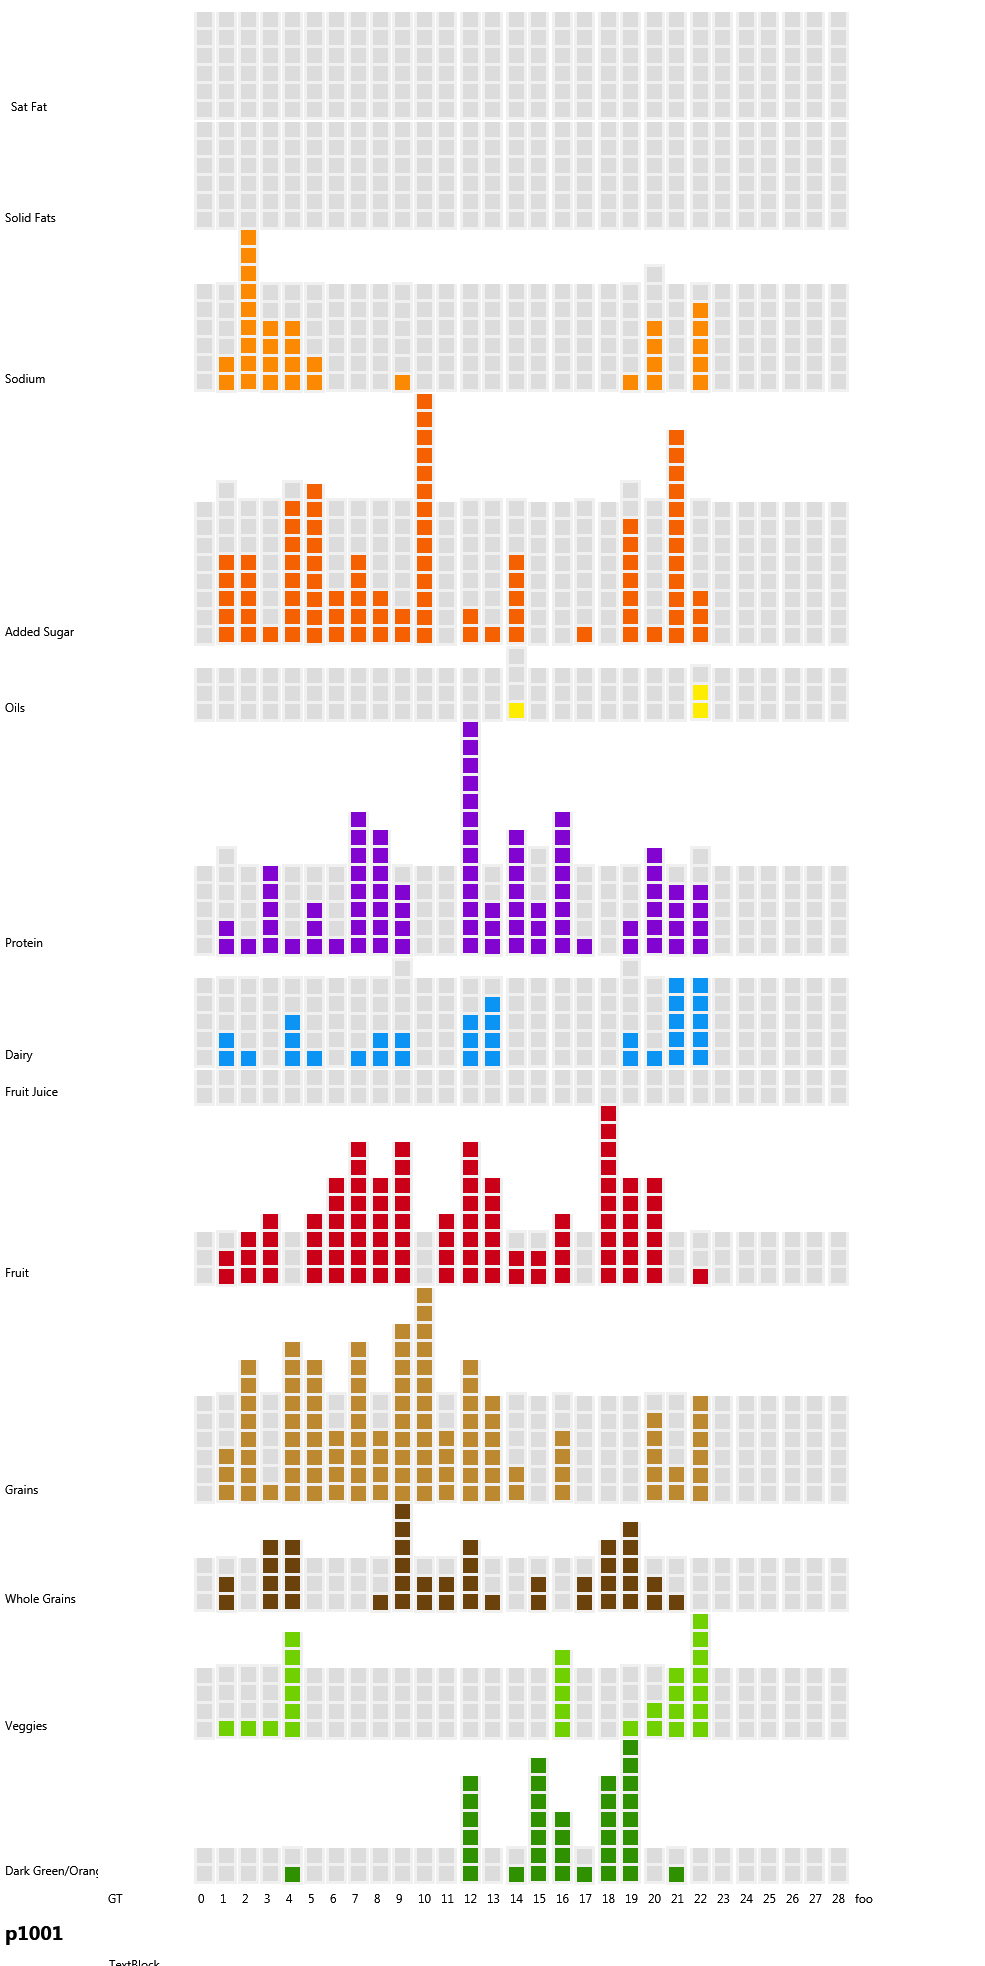
\includegraphics[ height=5in ]{./images/cont4/ppt_overview}}
\label{fig:ppt_overview}

\caption{Overview of Ppt 1001}
\end{center}
\end{figure}


% Table generated by Excel2LaTeX from sheet 'Sheet11'
\begin{sidewaystable}[htbp]
\small
  \centering
  \caption{Final Component Counts}
    \begin{tabular}{rrrrrrrrrrrrr}
    \toprule
    \rotatebox{45}{Ppt ID} & \rotatebox{45}{Fruit Juice} & \rotatebox{45}{Fruit} & \rotatebox{45}{Veggie} & \rotatebox{45}{\parbox{2.5cm}{Dark Green \&\\Orange Veggie}} & \rotatebox{45}{Grains} & \rotatebox{45}{\parbox{1.5cm}{Whole \\Grains}} & \rotatebox{45}{Protein} & \rotatebox{45}{Dairy} & \rotatebox{45}{Sodium}  & \rotatebox{45}{Sugar}  & \rotatebox{45}{Solid Fats} & \rotatebox{45}{Oils} \\
    \midrule
    p1001 & 2.5   & 8.0   & 28.0  & 11.0  & 57.5  & 14.0  & 66.0  & 46.0  & 61.5  & 47.0  & 31.0  & 12.0 \\
    p1003 & 0.0   & 89.0  & 27.0  & 35.0  & 102.0 & 41.0  & 80.0  & 29.0  & 29.5  & 81.5  & 0.0   & 2.5 \\
    P1004 & 6.0   & 13.5  & 14.0  & 3.5   & 25.0  & 21.5  & 29.0  & 21.0  & 1.0   & 21.0  & 4.6   & 2.5 \\
    p2001 & 0.0   & 1.0   & 11.0  & 2.0   & 30.0  & 0.0   & 11.0  & 2.5   & 31.0  & 14.5  & 20.9  & 2.0 \\
    P2002 & 0.0   & 17.5  & 24.0  & 12.0  & 74.5  & 20.0  & 56.0  & 44.5  & 66.0  & 54.5  & 62.8  & 34.0 \\
    p3002 & 4.0   & 24.5  & 15.5  & 4.0   & 37.0  & 8.0   & 24.5  & 33.5  & 22.5  & 37.5  & 10.6  & 2.0 \\
    P3011 & 3.0   & 0.0   & 32.5  & 12.0  & 44.7  & 20.5  & 29.0  & 21.0  & 63.2  & 39.2  & 55.1  & 34.5 \\
    p3012 & 5.0   & 9.5   & 41.0  & 19.0  & 32.5  & 17.0  & 50.5  & 20.0  & 15.5  & 44.0  & 37.0  & 10.0 \\
    P3013 & 3.0   & 54.0  & 48.0  & 55.5  & 3.0   & 29.0  & 107.0 & 63.5  & 0.0   & 2.0   & 1.0   & 13.0 \\
    p3014 & 2.0   & 21.0  & 33.0  & 30.0  & 28.0  & 53.0  & 58.0  & 44.0  & 26.0  & 16.0  & 30.0  & 14.0 \\
    p3021 & 3.0   & 31.0  & 68.0  & 61.5  & 68.0  & 26.0  & 220.0 & 58.5  & 118.7 & 63.2  & 97.7  & 71.0 \\
    p3022 & 13.0  & 20.0  & 18.5  & 7.0   & 83.5  & 14.0  & 40.0  & 58.6  & 77.1  & 75.3  & 80.8  & 12.0 \\
    P3023 & 4.0   & 19.5  & 29.4  & 14.0  & 33.3  & 32.0  & 44.3  & 30.0  & 22.3  & 28.3  & 34.5  & 12.0 \\
    P3024 & 30.0  & 17.5  & 13.0  & 5.0   & 52.5  & 1.0   & 19.0  & 18.0  & 78.9  & 31.3  & 30.0  & 0.0 \\
    p4001 & 4.0   & 46.5  & 39.0  & 51.5  & 31.5  & 74.5  & 67.0  & 45.0  & 60.5  & 29.0  & 52.4  & 54.0 \\
    p4002 & 0.0   & 27.0  & 65.0  & 0.0   & 47.0  & 68.0  & 56.5  & 49.0  & 88.0  & 1.0   & 15.0  & 20.0 \\
    P4003 & 27.0  & 18.5  & 48.0  & 0.0   & 0.0   & 44.5  & 67.5  & 49.0  & 1.5   & 119.5 & 8.6   & 0.0 \\
    p5001 & 14.0  & 18.0  & 22.5  & 17.5  & 110.9 & 4.0   & 61.5  & 48.0  & 47.4  & 104.9 & 51.1  & 1.0 \\
    p5002 & 0.0   & 13.0  & 18.5  & 15.0  & 8.5   & 0.0   & 36.5  & 10.5  & 25.0  & 7.5   & 5.5   & 12.0 \\
    p5003 & 1.0   & 38.0  & 21.0  & 27.0  & 49.0  & 51.0  & 37.0  & 63.0  & 34.5  & 28.0  & 42.3  & 22.0 \\
\midrule
    Mean  & 6.1   & 24.4  & 30.8  & 19.1  & 45.9  & 27.0  & 58.0  & 37.7  & 43.5  & 42.3  & 33.6  & 16.5 \\
\midrule
    Target  & 42   & 63  & 84  & 42  & 126  & 63  & 105  & 105  & 126  & 168  & 126  & 63 \\
    \bottomrule
    \end{tabular}%
  \label{tab:insituComponentCounts}%
\end{sidewaystable}%


\subsubsection{Guided Interview}
At the end of the study, participants returned to the lab to conduct an in-person semi-structured interview about their use of the tool. The interview protocol is attached as an appendix, as is the coding documentation. Below, I report some of the responses to selected questions. 

\textbf{Were you able to make food entries right after you ate? When you were not able, why not?}
This question resulted in a wide range of responses. Some people reported using it consistently after eating, while others made comments that some meals were easy to remember to enter because they are at times that their routine is consistent or predictable; other meals were at times when the routine is unpredictable. Participants also commented about how their schedules changed week to week: participants who had been traveling noted that their schedules were just off overall. Some people changed schedules over the study: one participant noted that there was one week of classes that was ``predictably crazy'', one week of vacation that was relaxed and easy to pay attention, and one week of starting an internship rotation in a venue that was high-pressure and busy, where it was hard to remember or want to think about entering. Other issues that prevented people from making entries immediately after eating included that their phone wasn't with them (frequently commented that it was elsewhere, charging) or they were doing something else while eating and forgot. 

\textbf{What were 3 things you really liked about this diary?}
Many comments were about what features people would like. An improved food database and searching process were frequently mentioned. People also wanted to track their water intake, and some people wanted some notion of calorie intake. In regards to calories, some people wanted detailed caloric information, while others reported being comfortable with an estimate. People also talked about wanting more customization: the order of the items on the screen, the background color, which items appear on the front screen. A couple of people volunteered the notion of a ``Junk food'' button-to indicate that they had something with low nutritional value, but with less detail than specifying how much sugar, salt, or fat it contains. 

Our participants liked the distinction between whole grains and refined grains, and dark green/orange vegetables and all other vegetables. They also liked the overview or analysis this approach provided. The color coding of the different components appeared to support the analysis. Many people had trouble tracking sugar, sodium and fats, which is consistent with previous work of tracking nutrients. Due to this, some people chose to ignore the nutrients. In addition to the inherent challenge of tracking nutrients, some participants noted philosophical objections to monitoring the nutrients. One participant expressed concern about current nutrition recommendations to drastically restrict fat and salt. Other participants expressed a perspective that being too concerned about the accuracy of the nutrients in particular could reflect an unhealthy obsession. 

When asked about things people didn't want to record, one response was ``things I wasn't sure how to spell''. 

\textbf{Was there a pattern, rule or guideline you used to decide when to search for a food rather than enter it via ``+1''s? }
Participants reported three primary approaches to creating entries. Some participants preferred looking foods up in the database, but ended up using the +1 feature due to difficulties  in the lookup process. Difficulties included: uncertainty of what phrase to use to find the food; inability to find a food they wanted; not trusting the results of the database (e.g., Subway sandwich with no grains); and occasional software malfunction. One participant reported consistent software crashes when looking up food in the database. This participant resorted to using the +1 buttons to continue study participation, but reported preferring the lookup. Other participants chose to use the +1 feature as much as possible. Finally, some participants took the approach of looking up anything that was packaged, ``had a barcode'', or prepared at a restaurant, while using the +1 for anything self-prepared. 

\textbf{Are you currently satisfied with your nutrition behaviors?}
The first few interviews revealed that our participants had different self-assessments of their eating behaviors. This question was added in to attempt to capture this information from all participants. Some participants demonstrated a high degree of nutritional literacy and felt confident that their eating behaviors reflected this knowledge most of the time. Others demonstrated nutritional literacy, but indicated that they knew their current eating behaviors were not consistent with known recommendations. Finally, some participants did not reflect awareness or concern about their eating behaviors in general. 

\textbf{Did keeping a food record change how you ate? How so?}
Some people talked about how the tool helped them to think more about the choices they were making, and they ended up eating more whole grains, choosing more vegetables, eating or buying more fruits, or choosing not to eat something that would increase the yellows and orange categories. Some people were surprised about some of the nutrients they encountered: things like sugar in slushy, sodium in soup, or that they really did not consume as many whole grains as they believed they did. 


\textbf{Would you recommend POND to friends? Are there other people you would recommend this tool to?}
When asked who they would recommend this tool to, many people volunteered that it would be really good for senior citizens, because it is so easy to use and keeps things so simple. Others indicated that they thought it would be good for busy mothers and caregivers, not just to track for themselves but to also keep track of what children (or family members) eat. They felt POND could support communication about nutrition behaviors among all family members. People also thought it might be good for people who were just starting to try to figure out how to make changes in their diet. Two participants felt that POND would  not be useful for anyone because it did not provide enough detailed information. These two participants later reported concern about specific carbohydrate counts and calorie counts, respectively. Other participants thought POND could be useful to anyone, because it is simple, provides high level feedback,  and supports awareness of one's dietary patterns. 

\textbf{Did you use the location tagging feature? }
We asked people to volunteer coarse location information for entries. No one did so. In general, the feedback on this feature was that participants did not believe location mattered. Their perspective was that they did not care about analyzing where they ate food, and it was just another thing to do, so they chose not to do it. A couple of people volunteered that they might be able to imagine there are patterns in the data, but they did not think there was likely any insight or value from it. 

\textbf{Why did you choose to participate in this study?}
Finally, I asked participants why they participated in the study. Some people did it purely for personal interest, stating that generally they are interested in tools to support their own health and wellness, while others did it just for the money. A couple of people had a balance of the two. 

One area of confusion was not directly identified by a question, but emerged in the interview. 
Many participants were unclear if the goals were to be attained or moderated. The POND interface design specifically did not reflect this. The design rationale was that when POND is used in the greater context of a goal-oriented dietary change program, the goals would be personal and self-identified. Therefore, the user would know whether an individual component goal was to be attained or moderated. Since this trial did not directly evaluate the goal-tending support, the lack of an indicator was problematic. The Fruit Juice component was particularly confusing: some participants noted that they do not usually consume fruit juice, and they were not sure if the dietary guideline was making the recommendation to drink more juice. In fact, the guideline was to restrict juice intake, but when juice is chosen, ensure that it is 100\% juice. 


\subsection{Discussion}
The goal of the \textit{in situ} POND evaluation was to characterize how people used the POND software to monitor the foods they eat in the context of their daily lives. We looked at how often people used the +1 buttons to make an entry rather than looking up a food in the database, the searches that were made and reported on search characteristics, the total number of components that were entered overall, how many entries were made each week, and what participants told us about their routines throughout the study period. 

Nine participants used the food lookup on a regular basis. However, no one refused to make entries with the +1 buttons, even if they reported preferring the feeling of accuracy associated with using the lookup feature. This could indicate that people found the +1 approach beneficial at least part of the time. 

As in the in-lab study, we see that the commonly performed searches include foods that are difficult for people to know how to count in terms of the HEI components. 

The frequency of the search for `egg' reflects a problem with the ``Protein'' category. The category is formally called ``Meat, Beans, and Eggs'', but we made a design decision to shorten the title to ``Protein'' to fit the mobile device screen better. This resulted in participants expressing confusion about the Protein category. Participants reported counting protein bars and protein powder under the ``Protein'' category. The appropriateness of counting protein bars and powders in the Protein category depends on the source of the protein: Whey protein is a dairy derivative, while soy protein comes from beans. Another way the Protein category caused confusion was in terms of serving size. Protein is a macronutrient, and is reported on nutrition labels in grams. The HEI ``Meat, Beans and Eggs'' category (called Protein in POND) is to be counted in terms of ounces of meat, number of eggs, or servings of beans. Since one ounce of meat has about 7 grams of protein, mistakenly counting `grams of protein' rather than `ounces of meat' can lead to bad numbers. 

The overall component counts for each participant show that people probably did not count the nutrients correctly. The nutrients (sodium, sugar, solid fats, oils) are also moderation components, which means that in general, most people eat too much of those items, and the HEI recommends working to moderate one's intake of these items. However, all of the counts are quite low in relation to the targets. Although the target amounts may be high for this population, it is more likely that participants focused on the easy to use +1 buttons for counting the food group components. This is consistent with the entry strategy results, which showed more use of the +1 buttons than the lookup approach. This is also consistent with what participants reported in the final interview-- that the nutrient components were challenging to count. 

The final interviews revealed that many participants were confused about the target amounts. Although it was addressed in the initial launching of the study, participants were not always sure if all of the targets were to be attained or moderated. Additionally, some participants seemed to think that some of the components were not defined properly. One participant in particular was concerned about the protein target, in regards to the concerns discussed earlier. The concern about the targets is reasonable, as they were defined based on a ``typical'' American who requires 2000 calories each day. The targets were not modified for individuals, and as many of our participants were adult women, it is likely the targets were too high for them. 

The interview asked people to report on how typical their schedules and routines were over the study period. Some people reported fairly consistent routines that were typical, while others reported that some of the weeks were inconsistent and atypical (going on vacation, starting a new job). Most participants were able to characterize when they were able to consistently make food entries in a timely manner (that is, shortly after eating), and it usually had to do with their routine. However, each person had different characteristics about their routine that made it easy or challenging to make timely entries: some people were very busy at work, but structured at home; for others it was the opposite. Given the opportunity, no one chose to track the location of where they were making entries. This is interesting, because participants reported not wanting to track location because they did not think it would be an informative or useful piece of information. However, from a research or design perspective, what they were telling us was that their ability to make entries depending on their location. 

\section{Overall POND Observations and Discussion}
The POND evaluation included two phases: an in-lab phase where we could focus on the use of the POND app to enter known food items, and an \textit{in situ} phase where we could better understand how POND performed as a self-monitoring tool within the context of a user's real life. In both phases, we looked at how people created entries (using the +1 buttons or looking foods up in the database); what searches were made; and what components people focused on and used to make entries. 


\subsection{How}
I first looked at the strategies people used to create food entries. This could be either the streamlined +1 strategy, or the more detailed, accurate lookup strategy. 

The in-lab data indicated that individuals fall into one of three groups: those that value the quick and easy overview entry, those that value the accuracy of the lookup, and those that are willing to combine strategies. In the context of the real world, we see that more people default to the use of the +1 entries. Generally, we saw that participants (consistent with what they reported) used the lookup feature to enter processed and prepared foods. Also, participants in the in-lab study made 650 queries to look up 4 days of food, while for the entire 3-week study, only 465 queries were made. The increased reliance on the +1 buttons and the small number of queries made could reflect a growing familiarity with the counting scheme, as well as being more familiar with the food one eats in general (as opposed to the food in the tasks that could be less familiar). 

\subsection{What}
I next looked at what entries people made. In the in-lab portion of the study, the foods were defined. This means that the users had no control over what to enter into the software. Instead, I look at what queries they made when they chose to use the food lookup feature. I could compare the queries made in the in-lab study to those from the \textit{in situ} study. 

When we look at the queries that people made in the in-lab versus \textit{in situ} conditions, the \textit{in situ} searches were shorter (mean = 10.03 versus 13.6 characters, longest = 35 versus 40 characters). This could reflect that participants were more familiar with the foods they were eating, and not impacted by the long given names in the in-lab tasks. 

It is challenging to identify what foods were entered in the \textit{in situ} study. Some participants made entries via lookup, but most participants did not make most entries via lookup. They used the +1 approach instead. For this discussion, I look at the final component counts to reflect what participants entered into the software. 

The final component counts show that participants probably did not make the nutrient (sugar, sodium, solid fats, oils) entries consistently. Some people specifically chose to remove these components from the list of goals and not monitor them, while others may have decided that they were not worth the effort to monitor. User feedback indicates that even when participants thought these nutrients were worth monitoring, they chose not to because it was too challenging. However, consistent with the previous in-lab study, people seem to want a reminder of the components that they should moderate (restrict), even if they decide they do not want to actively monitor it. 

\subsection{When}
Finally, I looked at when participants made entries. This included both timestamps of entry creation and self-report of when participants made entries. 

The feedback from participants about when they made entries, and when it was challenging to make entries, was valuable. The focus group feedback from BALANCE revealed that people wanted to use small stretches of time when they were not doing much else to create food diary entries. There were a number of reasons for this. However, feedback from the POND study indicates that users were willing to make time for creating entries, as long as they could fit it into their schedule. That is, when participants had consistent, predictable schedules, users made time to create food entries. When the schedule was less predictable or consistent, users found it difficult to remember to create food entries at the time of eating. 

\subsection{Overall}
Participants in the \textit{in situ} study reported that using the POND software made them more aware of the processed foods that they ate. This appeared to include both which eaten foods were processed and how many processed foods they ate overall. Participants reported using the food lookup feature more frequently for processed or prepared foods, and the +1 feature for entering foods they prepared themselves. User awareness of their consumption of processed foods is important because people in general tend to be unaware of how many processed foods they eat. Processed foods also tend to contain more salt, sugar and fat than self-prepared foods. Participants in the POND study reflected surprise at the nutritional content of prepared foods. In particular, the component-based visualization appeared have more impact than the same numbers reported on the nutrition label of a food. A processed food entry such as a Slushie would show on the list of components as many sugar blocks, but no other blocks. This helped to put into perspective how processed foods impacted the moderation goals, but had no impact on the attainment goals. 

The component-based approach of analyzing processed foods helped participants to better understand what a given food was composed of. One example to note is that of Doritos, a food in one of the in-lab tasks. Sometimes participants noted that they were not sure how to count Doritos. Doritos happen to consist of a grain (corn), fat and salt. This awareness could help build nutritional literacy over time. This is consistent with participants who suggested that POND would be a good tool for people just learning about nutrition or just beginning a dietary change program. 

The awareness of processed versus self-prepared foods is one reason participants liked the overview analysis the POND tool presented. Participants noted that the visual nature of the gray and colored blocks helped them to stay aware of their overall consumption over time. Users became more aware of when their fruit and vegetable intake fluctuated. Touching the +1 button to declare that they ate ``something healthy'' was considered satisfying. In particular, one participant noted that she preferred the lookup strategy to ensure the accuracy of her diary, but she appreciated that the overview visualization allowed her to ensure that her dietary intake was well-balanced. 

Burke et al \citep{burke_experiences_2009} found that participants in a study focused on the impact of self-monitoring as part of a weight loss program fell into three groups: highly involved, nominally involved, and negligibly involved. In contrast, the participants in the POND study were all either nominally involved  or highly involved in the self-monitoring process. This difference could be related to the distinction of self-monitoring as part of a weight loss program, or due to the alternative input strategy that POND provided. 

Early evaluation shows that POND appears to support various user characteristics. Follow-on work will incorporate a more rigorous quantification of those characteristics. Next steps for the POND project include evaluating its use by participants with specific, stated goals and in specific stages of change as defined by the transtheoretical model \citep{prochaska_transtheoretical_1997}. 

\section{Summary}
In this chapter I described the evaluation of the POND food diary. The evaluation consisted of both in-lab and \textit{in situ} parts. An initial analysis focused on how participants made entries, what they made entries of, and when they made entries. I found that participants had preferences for either detailed, accurate records and were willing to take the time to look foods up in the database, or were satisfied with the overview analysis and only used the +1 buttons. Participants appreciated that the +1 buttons made the process to enter some foods easier and faster. Participants also provided rich descriptions of the context of when they were able to make entries, or when there were barriers to making entries. 
